\documentclass[aspectratio=169,12pt]{beamer}
\usepackage[T1]{fontenc} %pipes don't display properly without this
\usepackage[utf8]{inputenc}
\usepackage{listings}
\usepackage{color}
\usepackage{datapie}
\usepackage{multicol}
\usepackage{siunitx} %pretty measurement unit rendering
\usepackage{hyperref} %enable hyperlink for urls
\usepackage{caption} % needed to tweak caption size

\usefonttheme[onlymath]{serif}
\setcounter{MaxMatrixCols}{20}

\DeclareSIUnit\pixel{px}

\usecolortheme[RGB={37,68,113}]{structure}
\usetheme{Dresden}

\newenvironment{figurehere}
{\def\@captype{figure}}
{}
\makeatother

%commands to exclude sections from miniframes
\makeatletter
\let\beamer@writeslidentry@miniframeson=\beamer@writeslidentry
\def\beamer@writeslidentry@miniframesoff{%
   	\expandafter\beamer@ifempty\expandafter{\beamer@framestartpage}{}% does not happen normally
   	{%else
   		% removed \addtocontents commands
   		\clearpage\beamer@notesactions%
   	}
}
\newcommand*{\miniframeson}{\let\beamer@writeslidentry=\beamer@writeslidentry@miniframeson}
\newcommand*{\miniframesoff}{\let\beamer@writeslidentry=\beamer@writeslidentry@miniframesoff}
\beamer@compresstrue
\makeatother


\providecommand{\tightlist}{%
  \setlength{\itemsep}{0pt}\setlength{\parskip}{0pt}}


%various gray colors
\definecolor{slg}{gray}{0.25}
\definecolor{lg}{gray}{0.55}
\definecolor{vlg}{gray}{0.73}
\definecolor{tlg}{gray}{0.9}

%TheAlt colors
\definecolor{ldorange}{HTML}{F18A20}
\colorlet{ldbright}{ldorange!70!white} % tinted version of orange, used in miniframes
\definecolor{ldblue}{HTML}{254471}

%reduce caption font size:
\captionsetup{font={scriptsize,color=lg}}

%do not prepend numbering/lettering to figures/subfigures
\captionsetup{labelformat=empty} %do not prepend letters to figure captions

%Apply TheAlt colors to theme
 % section titles in top navigation bar
\setbeamercolor{section in head/foot}{parent=palette tertiary,fg=ldorange}
\setbeamertemplate{section in head/foot shaded}{\color{ldbright}\usebeamertemplate{section in head/foot}}
 % miniframes (little navigation circles)
\setbeamercolor*{mini frame}{fg=ldorange,bg=ldbright}
\setbeamertemplate{mini frame in other section}[default][0]
\setbeamertemplate{mini frame in other subsection}[default][0]
 % others
\setbeamercolor{author in head/foot}{fg=white}
\setbeamercolor{subsection in head/foot}{fg=white}
\setbeamercolor{caption name}{fg=vlg}
\setbeamercolor{caption}{fg=vlg}
\setbeamercolor{frametitle}{fg=ldblue}

\setbeamertemplate{caption}{\raggedright\insertcaption\par}
\setbeamertemplate{navigation symbols}{}
\setbeamertemplate{bibliography item}[text]

\definecolor{mygreen}{rgb}{0,0.6,0}
\definecolor{mygray}{rgb}{0.5,0.5,0.5}
\definecolor{mymauve}{rgb}{0.58,0,0.82}

\lstdefinestyle{custombash}{
	belowcaptionskip=1\baselineskip,
	captionpos=,
	breaklines=true,
	frame=L,
	xleftmargin=\parindent,
	language=bash,
	showstringspaces=false,
	basicstyle=\scriptsize\ttfamily,
	rulecolor=\color{tlg},
	backgroundcolor=\color{tlg},
	fillcolor=\color{tlg},
	rulesepcolor=\color{tlg},
	commentstyle=\itshape\color{purple!60!black},
	keywordstyle=\bfseries\color{ldorange!80!black},
	%keywordstyle=\bfseries\color{green!40!black},
	identifierstyle=\color{blue},
	stringstyle=\color{orange},
}

\lstset{language=Bash,style=custombash,caption={Descriptive Caption Text},label=DescriptiveLabel}


\institute{
\includegraphics[width=0.35\textwidth]{img/logo_blue.pdf}}
\date{}

\renewcommand{\emph}[1]{\textcolor{ldorange}{#1}}
\newcommand{\soft}[1]{\textcolor{lg}{#1}}
\newcommand{\textt}[1]{\textcolor{blue}{\texttt{#1}}}
\newcommand{\bigtext}[1]{\centering\Huge \textbf{\textcolor{ldorange}{#1}}}

%shortcut to insert small logo in footline
\def\logo{%
	\resizebox{!}{3ex}{
\includegraphics{img/logo_white.pdf}}
}

% Define a custom footline that includes our logo
\setbeamertemplate{footline}
{%
	\begin{beamercolorbox}[wd=\paperwidth,ht=2.5ex,dp=1.125ex,%
		leftskip=.3cm,rightskip=.3cm plus1fil]{title in head/foot}
		\usebeamerfont{title in head/foot}%
		\insertshorttitle\hfill\insertframenumber
	\end{beamercolorbox}
	\begin{beamercolorbox}[wd=\paperwidth,ht=3.5ex,dp=1.625ex,%
		leftskip=.3cm,rightskip=.3cm plus1fil]{author in head/foot}
		\usebeamerfont{author in head/foot}
		\raisebox{0.5ex}{\insertshortauthor}\hfill\raisebox{-0.5ex}{\logo}
	\end{beamercolorbox}
}

\begin{document}




\begin{frame}

\% Habits \% John Doe \% March 22, 2005

\end{frame}

\section{In the morning}

\subsection{A story}

\begin{frame}[fragile]{First some code}

\begin{verbatim}
echo "Hello World"
\end{verbatim}

\end{frame}

\begin{frame}{Getting up}

\begin{itemize}
\tightlist
\item
  Turn off alarm
\item
  Get out of bed
\end{itemize}

\end{frame}

\begin{frame}{Breakfast}

\begin{itemize}
\tightlist
\item
  Eat eggs
\item
  Drink coffee
\end{itemize}

\end{frame}

\section{In the evening}

\subsection{Another story}

\begin{frame}{Dinner}

\begin{itemize}
\tightlist
\item
  Eat spaghetti
\item
  Drink wine
\end{itemize}

\end{frame}

\begin{frame}{Going to sleep}

\begin{itemize}
\tightlist
\item
  Get in bed
\item
  Count sheep
\end{itemize}

\% Why CLI tools? \% Philip Stark, Nils Leuzinger \% 25 Oct, 2016

\end{frame}

\section{Very close integration with command line}

\subsection{Some particularly fancy features}

\section{Vim Basics}

\subsection{What Vim Is And Isn't}

\begin{frame}[fragile]{Vim is an editor}

\begin{verbatim}
...but probably unlike anything else you've ever used. 
And extremely powerful.
\end{verbatim}

\end{frame}

\begin{frame}[fragile]{Configurability}

\begin{verbatim}
Vimscript
- Remap keys
- Write whole plugins!
\end{verbatim}

\end{frame}

\subsection{Modal Editing}

\begin{frame}[fragile]{Vim Modes}

\begin{verbatim}
- Insert Mode
- Visual Mode
- Command-Line Mode
- Normal Mode
\end{verbatim}

\end{frame}

\begin{frame}[fragile]{Insert Mode}

\begin{verbatim}
Does what any other editor does
\end{verbatim}

\end{frame}

\begin{frame}[fragile]{Visual Mode}

\begin{verbatim}
Selecting text
\end{verbatim}

\end{frame}

\begin{frame}[fragile]{Command-Line Mode}

\begin{verbatim}
- Execute built-in vim commands
- Execute any shell command!
\end{verbatim}

\end{frame}

\begin{frame}[fragile]{Normal Mode}

\begin{verbatim}
Magic and hjkl.
\end{verbatim}

\end{frame}

\begin{frame}{}

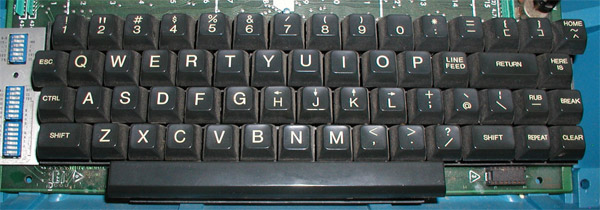
\includegraphics{resources/vim/hjkl_keyboard.jpg}\{ width=50\% \}

\end{frame}

\section{Getting Faster}

\subsection{Learning Vim}

\begin{frame}[fragile]{How To ``Grok'' Vim}

\begin{verbatim}
Some basic vim terminology:
- Verbs
- Motions
- Objects
\end{verbatim}

\end{frame}

\begin{frame}[fragile]{Productivity Tips}

\begin{verbatim}
Unmap the arrow keys.
Learn something new from time to time.
Actively try to improve your editing.
Tabs, Splits
Ctrl-Z
Watch some talks online: "Write Code Faster: Expert-Level Vim"
Learn Vimscript the Hard Way.
\end{verbatim}

\end{frame}

\section{Plugins}

\subsection{Plugins}

\begin{frame}[fragile]{Vim Is not an IDE}

\begin{verbatim}
But it can be. (Almost)
\end{verbatim}

\end{frame}

\begin{frame}{NERDTree}

\end{frame}

\begin{frame}{FileType}

\end{frame}

\begin{frame}{nerdcommenter}

\end{frame}


\end{document}
